\documentclass[a4paper,12pt]{extarticle}
\usepackage{geometry}
\usepackage[T1]{fontenc}
\usepackage[utf8]{inputenc}
\usepackage[english,russian]{babel}
\usepackage{amsmath}
\usepackage{amsthm}
\usepackage{amssymb}
\usepackage{fancyhdr}
\usepackage{setspace}
\usepackage{graphicx}
\usepackage{colortbl}
\usepackage{tikz}
\usepackage{pgf}
\usepackage{subcaption}
\usepackage{listings}
\usepackage{indentfirst}
\usepackage[colorlinks,citecolor=blue,linkcolor=blue,bookmarks=false,hypertexnames=true, urlcolor=blue]{hyperref} 
\usepackage[noabbrev]{cleveref}
\usepackage{indentfirst}
\usepackage{mathtools}
\usepackage{booktabs}
\usepackage[flushleft]{threeparttable}
\usepackage{tablefootnote}
% \usepackage{refcheck}

\usepackage{chngcntr} % нумерация графиков и таблиц по секциям
\counterwithin{table}{section}
\counterwithin{figure}{section}
\DeclareMathOperator*{\argmin}{arg\,min} 
\graphicspath{{graphics/}}%путь к рисункам

\makeatletter
\renewcommand{\@biblabel}[1]{#1.} % Заменяем библиографию с квадратных скобок на точку:
\makeatother

\geometry{left=2.5cm}% левое поле
\geometry{right=1.5cm}% правое поле
\geometry{top=1.5cm}% верхнее поле
\geometry{bottom=1.5cm}% нижнее поле
\renewcommand{\baselinestretch}{1.25} % междустрочный интервал
\RequirePackage{float}                


\addto\captionsrussian{\def\refname{Список литературы (или источников)}} 

\renewcommand{\theenumi}{\arabic{enumi}.}% Меняем везде перечисления на цифра.цифра
\renewcommand{\labelenumi}{\arabic{enumi}.}% Меняем везде перечисления на цифра.цифра
\renewcommand{\theenumii}{\arabic{enumii}.}% Меняем везде перечисления на цифра.цифра
\renewcommand{\labelenumii}{\arabic{enumi}.\arabic{enumii}.}% Меняем везде перечисления на цифра.цифра
\renewcommand{\theenumiii}{\arabic{enumiii}.}% Меняем везде перечисления на цифра.цифра
\renewcommand{\labelenumiii}{\arabic{enumi}.\arabic{enumii}.\arabic{enumiii}.}% Меняем везде перечисления на цифра.цифра

\crefname{figure}{рис.}{рис. }
\Crefname{figure}{Рис.}{Рис. }
\crefname{table}{табл.}{табл. }
\Crefname{table}{Табл.}{Табл. }

\begin{document}
\begin{titlepage}
    \newpage
    
    {\setstretch{1.0}
    \begin{center}
    Федеральное государственное автономное образовательное \\
    учреждение высшего образования \\
    \vspace{1em}
    <<Национальный исследовательский университет \\
    <<Высшая школа экономики>>
    \\
    \vspace{4em}
    Факультет компьютерных наук \\
    \vspace{1em}
    Основная образовательная программа \\
    Прикладная математика и информатика \\
    \end{center}
    }
    
    \vspace{10em}
    
    \begin{center}
        \textbf{КУРСОВАЯ РАБОТА}
        \vspace{2em}
        \\
        \textbf{
            Программный проект на тему
            \linebreak
            <<Сервис поиска соседних объектов>>
        }
    \end{center}
    
    \vspace{8em}
    
    {\setstretch{1.0}
    \hfill\parbox{16cm}{
    \hspace*{5cm}\hspace*{-5cm}Выполнил студент группы БПМИ 195, 3 курса,\\
    Амеличев Константин Вадимович\\
     
    \hspace*{5cm}\hspace*{-5cm}Руководитель КР:\\
    Руководитель группы разработки, Tinkoff.ru, Тощев Андрей Александрович\\
    
    %\hspace*{5cm}\hspace*{-5cm}Куратор:\hfill < степень>, <звание>, <ФИО полностью>\\
    }
    }
    
    \vspace{\fill}

\begin{center}
Москва 2022
\end{center}
    
\end{titlepage}% это титульный лист
\newpage

{
	\hypersetup{linkcolor=black}
	\tableofcontents
}

\newpage



\section{Аннотация}

В рамках курсовой работы описывается исследование задачи поиска ближайших соседей и разработка поискового сервиса SimSearch. SimSearch позволяет находить объекты, максимально похожие по свойствам на запрошенный пользователем объект. Описывается возможность реализовать поисковое приложение для любого типа объектов, у которых определена функция перевода их характеристик в вектор: для изображений, документов, пользователей рекомендательной системы и прочего. Данный подход демонстрируется разработанным поиском похожих изображений на основе SimSearch.

\textbf{Ключевые слова:} Задача поиска ближайшего соседа, поисковые системы.

\hfill

The course work describes the study of the problem of finding nearest neighbors and the development of the search service SimSearch. SimSearch allows you to find objects that are most similar in properties to the object requested by the user. The possibility is described to implement a search application for any type of objects that have a function for translating their characteristics into a vector: for images, documents, users of a recommender system, and others. This approach is demonstrated by the developed search for similar images based on SimSearch.

\textbf{Keywords:} Nearest neighbor search, search engine.

\newpage

\section{Введение}

При работе с данными часто возникает необходимость в поиске некоторого элемента в имеющемся хранилище данных. В случае, если объекты в базе покрывают все возможные поисковые запросы, нужно искать точное совпадение в множестве. В случаях, когда база
фиксирована, а поисковое пространство неограниченно, принято искать не точное, а <<похожее>> совпадение: основные характеристики объектов должны либо совпадать, либо отличаться незначительно. Например, на <<похожих>> изображениях находятся объекты одного и того же класса: изображения двух разных чашек кофе считаются <<похожими>>, но изображение чашки кофе не похоже на изображение гоночного автомобиля.

В рамках работы произойдет переход от интуитивного определения <<похожести>> к более формальной поисковой задаче, где объектом выступит вектор, а <<похожесть>> окажется связано с расстоянием между векторами.

\subsection{Цель курсовой работы}

Целью курсовой работы является создание сервиса SimSearch (от англ. \textit{similarity search}), который будет находить объекты, <<похожие>> на объект, который запросил пользователь.

Важно заметить, что \textit{объект}~--- абстрактное понятие, и единственное требование, накладываемое на него в рамках данной работы~--- векторизуемость, переносящее метрику <<похожести>> в некоторое расстояние между двумя векторами. Чем меньше расстояние между векторами, тем более похожи объекты. Такая векторизация называется \textit{эмбеддингом} \cite{embedding}. Соответственно, разработанный сервис должен быть гибким и доступным для использования с различными поисковыми пространствами: от пользователя требуется только определить функцию перевода объекта в вектор и предоставить необходимые данные для поиска.

\subsection{Задача поиска ближайших векторов}

Опишем задачу поиска соседних векторов более подробно. Пусть объект описывается вектором $v = \begin{pmatrix}v_1 \\ v_2 \\ \ldots \\ v_d\end{pmatrix} \in \mathbb{R}^d$, а также у нас есть множество векторов $S~\subseteq \mathbb{R}^d$. Таким образом, $S$~--- это \textit{датасет} из $n$ векторов в $d$-мерном пространстве. Определим некоторое расстояние между векторами как $dist(v_1, v_2)$. Поиск <<достаточно близких>> векторов принято называть задачей $c$-ANN (Approximate Nearest Neighbors), где $c$~--- параметр задачи ($c > 1$). Положим $q$~--- искомый вектор, а $v^* = \displaystyle \argmin_{v \in S} dist(v, q)$. Таким образом, $v^*$~--- самый близкий вектор к запрашиваемому. Ответом на задачу $c$-ANN считается вектор $v$, удовлетворяющий неравенству:

$$dist(v, q) \le c \cdot dist(v^*, q)$$
\newpage
Обычно в качестве расстояний используется одна из следующих метрик:
\label{DIST}
\begin{itemize}

\item Евклидово расстояние: $dist(v_1, v_2) = \sqrt{\langle v_1 - v_2,v_1 - v_2\rangle}$
\item Косинусное расстояние: $dist(v_1, v_2) = \frac{\langle v_1, v_2\rangle}{\sqrt{\langle v_1, v_1\rangle \cdot \langle v_2,v_2\rangle}}$
\item Расстояние Минковского: $dist(v_1, v_2) = \displaystyle \sum_{i = 1}^d |v_{1, i} - v_{2, i}|$
\item Расстояние Джакарда: $dist(v_1, v_2) = 1 - \frac{\displaystyle \sum_{i = 1}^d [v_{1, i} = v_{2, i}]}{2 \cdot d - \displaystyle \sum_{i = 1}^d [v_{1, i} = v_{2, i}]}$

\end{itemize}

Такие расстояния, как расстояние Джакарда или расстояние Хэмминга (частный случай расстояния Минковского) принято использовать на булевых векторах, каждая координата которого равна либо 0, либо 1. Это связано с тем, что в некоторых случаях сложно трактовать <<численную близость>> векторов, и гораздо проще думать о задаче в бинарном виде, с подходом из теории множеств: единица соответствует наличию <<признака>>, а 0 его отсутствию. Подобный подход встречается, например, в машинном обучении, под названием One Hot Encoding \cite{ohe}.

Также есть понятие задачи $c$-$k$-ANN, где ответом является множество из $k$ различных векторов, каждый из которых является ответом на задачу $c$-ANN.

\subsection{Требования к SimSearch}

Кроме главного функционального требования, которое мы накладываем на SimSearch (решение задачи поиска соседних объектов), имеет смысл сформулировать дополнительные требования: необходимый функционал сервиса, возможные характеры нагрузки.

Функционал, помимо решения задачи поиска соседних объектов, включает в себя следующие пункты:
\begin{itemize}
    \item Одна инсталляция SimSearch поддерживает различные типы объектов независимым образом~--- например, поддерживается работа одновременно с изображениями и текстами.
    \item SimSearch является масштабируемым \cite{enwiki:1086627524}~--- он может быть запущен на нескольких серверах \cite{enwiki:1086236982}, которые будут пользоваться одной общей базой данных.
    \item SimSearch поддерживает запросы добавления, изменения и удаления объектов из множества.
    \item SimSearch имеет настраивыемые стратегии поиска объектов, выбор стратегий ложится на пользователя сервиса.
    \item SimSearch хранит не только информацию об объекте, необходимую для поиска, но и мета-информацию, которая может быть полезна пользователю сервиса.
\end{itemize}

Нагрузка может быть трех видов:
\begin{enumerate}
    \item Статическая: множество объектов для поиска фиксировано и не меняется. Может использоваться для данных, собранных разово и не меняющихся. Например, при построении систем для рекомендации классической литературы --- новые объекты в базе не появляются.
    \item Динамическая: множество объектов постоянно меняется, происходит добавление или удаление объектов. Общее ограничение на размер множества известно заранее. Например, это полезно для нахождения пользователей со схожими интересами и использования этих данных в рекомендательных системах.
    \item Нерегулярные изменения: множество объектов изменяется редко, но изменение или добавление затрагивает множество объектов. Такая нагрузка может обрабатываться так же, как и статическая, при массовых обновлениях достаточно просто заменить старое множество на новое. Такие обновления происходят редко, и можно перестроить базу с нуля, так что такая нагрузка будет обрабатываться так же, как и статическая.
\end{enumerate}

\subsection{Актуальность и значимость}

Идея поиска похожих объектов достаточно хорошо исследована для специфичных объектов (например, для изображений или текста). Сервисы, которые реализуют подобные поиски, обычно завязываются на специфику задачи, за счет чего перестают быть применимыми в других задачах.

Например, Shazam\cite{shazam} решает задачу поиска  похожих аудиозаписей~--- сервис находит фрагмент песни в поисковом индексе, максимально похожий на аудиофрагмент, записанный пользователем. Но подобный сервис нельзя использовать с другими типами данных, даже в похожих сценариях использования. Например, пользователь Shazam не может сфотографировать картину в музее и узнать, что это за картина, хотя поисковые задачи явно похожи друг на друга.

Есть и более нестандартные варианты. Например, существует веб-сервис для поиска других веб-сервисов \cite{ngu2014servicexplorer}, где объекты являются описанием веб-сервисов. Таким образом, можно найти онлайн-калькулятор или сервис для компьютерного перевода с английского на русский языки. Разумеется, подобный сервис не применим для любых других поисковых задач.

Сервисов же, которые решают универсальную поисковую задачу, не существует. В отличие от заточенных на специфичные объекты сервисов, SimSearch реализует некоторую общую логику и предлагает модель построения универсального поискового сервиса. Сервис, описываемый в данной работе, не завязывается на специфику объектов. Таким образом, поисковая задача разбивается на две подзадачи~--- задачу эмбеддинга \cite{embedding} и задачу поиска соседних векторов в многомерном пространстве.

SimSearch готовит для пользователя такую модель решения поисковой задачи, что при возникновении любой специфической задачи поиска, пользователю SimSearch нужно думать только о переводе задачи поиска соседних объектов в задачу поиска соседних векторов с помощью эмбеддинга. Непосредственно разработкой поискового движка заниматься не потребуется, так как за это отвечает SimSearch. Более того, для общей логики работы с часто встречающимися объектами (например, изображениями) эмбеддинги можно переиспользовать, что заметно ускоряет разработку прототипов нужных приложений.

Некоторые возможности для применения сервиса:
\label{SOLS}
\begin{enumerate}
\item Поиск референсов \cite{wiki:reference} в базе доступных картинок. Дизайнер, имеющий некоторое изображение, может найти похожее изображение, на которое у компании приобретены авторские права. Такое веб-приложение было разработано в рамках данной работы.
\item Рекомендательные системы. Зная, что пользователь А похож на пользователя B, можно предлагать пользователю B то, что понравилось пользователю A и не предлагать то, на что A отреагировал негативно. Таким образом, по критериям поиска можно определять аудиторию клиентов со схожими интересами. Всем представителям одной аудитории можно рекомендовать одинаковые или похожие интересные предложения.
\item Поиск песен, которые могут понравиться человеку на основе другой песни, которая ему уже нравится.
\end{enumerate}

Подробное изучение задачи эмбеддинга останется за рамками данной работы. Отметим, что для изображений можно использовать сверточные нейронные сети \cite{imageEmbeddings}, для аудиосигналов \cite{audiofingerprint}, рекомендательных систем \cite{barkan2016item2vec} и для текстов \cite{reimers2019sentence} также существуют свои эмбеддинги.

Можно заметить, что SimSearch не предлагает качество поиска выше, чем у специальных сервисов. Зато есть достаточно применений, в которых от сервиса нужно не столько хорошее качество сравнения, сколько отсев объектов, которые гарантированно не подходят под поисковый запрос. Например, такое актуально, когда поиск делается на небольших объемах данных. В терминах задачи $c$-$k$-ANN можно привести такой пример: пусть специализированный сервис решает задачу с параметром $c = 1.01$, а SimSearch решает эту же задачу с параметром $c = 1.02$. Тогда, с одной стороны, специализированный сервис давал погрешность вдвое меньшую, чем SimSearch. С другой стороны, на базах размером несколько тысяч объектов это не будет сильно отражаться на качестве поиска, в область со свойством $1.01 \cdot dist(v^*, q)) < dist(v, q) \le 1.02 \cdot dist(v^*, q)$ попадет мало объектов $v$, а значит, они не сильно ухудшат поисковую выдачу.

Главные преимущества использования SimSearch вместо специализированных сервисов:

\textbf{Гибкость.} SimSearch дает пользователю возможность невероятно гибкого использования. При решении конкретной поисковой задачи SimSearch предоставляет возможность гибко задать правила, влияющие на поисковую выдачу, ведь он разрешает настройку произвольного эмбеддинга и выбор нужной поисквовой стратегии.

Более того, мощность решаемых SimSearch поисковых задач упирается только в мощность эмбеддинга. Например, есть возможность создать две модели эмбеддинга ~--- первая переводит слова в пространство $\mathbb{R}^d$, вторая переводит изображения в пространство $\mathbb{R}^d$. Если модели на стадии обучения <<знали>> друг о друге и похожим объектам (картинке, похожей на свое текстовое описание) соответствуют похожие точки, то тогда поисковая задача для SimSearch окажется общей для двух типов. Например, это может быть полезно при получении изображения по текстовому описанию.

\textbf{Универсальность.} При регулярном решении различных поисковых задач поможет то, что у SimSearch одинаковый интерфейс для всех объектов, на которых ведется поиск. Таким образом, при возникновении задачи поиска в стороннем сервисе разработчику не потребуется искать новый поисковый сервис и делать с ним интеграцию. Это заметно уменьшает ресурсы на разработку, если разработчик решает задачу поиска сразу в нескольких вариациях.

\textbf{Переиспользование кода.} Если разработчик SimSearch добавил нестандартный алгоритм поиска (например, для какой-то необычной функции расстояния), он становится доступен всем остальным пользователям SimSearch, вне зависимости от объектов, для которых решалась поисковая задача. Таким образом, если в SimSearch существуют $n$ различных эмбеддингов и $m$ различных поисковых алгоритмов, то конфигурации сервиса можно настраивать по принципу <<каждый с каждым>>~--- всего $n \cdot m$ различных конфигураций. 

Сервис планируется использовать в качестве внутреннего поисковика для различных объектов финансового мобильного приложения ~--- изображений, иллюстрирующих <<истории>>, пользователей, ресторанов и прочего.

Сервис, похожий на SimSearch, был разработан в Google Cloud для демонстрации возможностей платформы Google Cloud Platform \cite{googlerealtimeembeddings}. Авторы реализуют сервис для семантического поиска в тексте, в некотором смысле делая связку между эмбеддингом текста в векторы и библиотекой для решения задачи $c$-$k$-ANN. Тем не менее, несмотря на похожую идею, авторами была решена конкретная поисковая задача для текстов, их решение не применимо для объектов другого типа.


\subsection{Задачи курсовой работы}

Разработанный сервис должен решать задачу $c$-$k$-ANN, иметь веб-интерфейс для взаимодействия с клиентами, а также поддерживать работу с несколькими типами хранилищ одновременно.

Таким образом, в данной курсовой работе решаются следующие задачи:

\begin{enumerate}
    \item Анализ задачи $c$-$k$-ANN и методов ее решения.
    \item Проектирование сервиса поиска соседних объектов.
    \item Разработка, отладка и тестирование SimSearch.
    \item Разработка веб-приложения для поиска похожих изображений на основе SimSearch.
    \item Описание полученных результатов в тексте курсовой работы.
\end{enumerate}

\newpage

\section {Обзор алгоритмов поиска}

Поскольку для решения задачи поиска соседних объектов нужен предварительный эмбеддинг, универсального способа решить задачу поиска не существует. В свою очередь, задача поиска ближайших векторов достаточно хорого изучена. Одна из задач работы --- сделать обзор существующих подходов, чтобы найти наиболее подходящий под задачу.

% Например, данная работа \cite{jafari2021survey} делает обзор имеющихся результатов в сфере локального хеширования. Авторы пишут, что для небольших размерностей используются структуры на основе деревьев (например, KD-дерево \cite{bentley1975multidimensional}). Для больших размерностей принято использовать locality-sensitive hashing \cite{gionis1999similarity}. У данного метода существует достаточно много вариаций и разновидностей.

\subsection{K-d деревья}

\label{KD}

Алгоритмы на основе деревьев \cite{enwiki:1089227535} разбивают поисковое пространство полуплоскостями в гиперпространстве. На \cref{ris:kdplane} можно посмотреть пример для пространства $\mathbb{R}^2$. K-d дерево --- двоичное дерево, которое строится над множеством объектов для поиска~--- каждый узел дерева содержит один вектор из множества. Дерево строится <<сверху вниз>>. Каждая новая вершина выбирается так, чтобы решить задачу разбиения: половина текущего множества вершин окажется в ее левом поддереве, другая половина~--- в правом поддереве. Для разбиения в самой тривиальной реализации можно использовать сравнение фиксированной координаты с соответствующей координатой вектора в вершине дерева. Таким образом, чтобы множество разбилось на две приблизительно равные части, сначала можно выбрать функцию, по которой вести сравнение (самое простое~--- выбрать одну из координат), а затем положить в вершину вектор из множества, который дает медианное значение функции. Полученная вершина разобьет множество на две части, и для них запустится рекурсивный процесс построения (\cref{ris:kdtree}). Итоговая глубина дерева получится равной $O(\log n)$.

\begin{center}
\begin{figure}[H]
\center{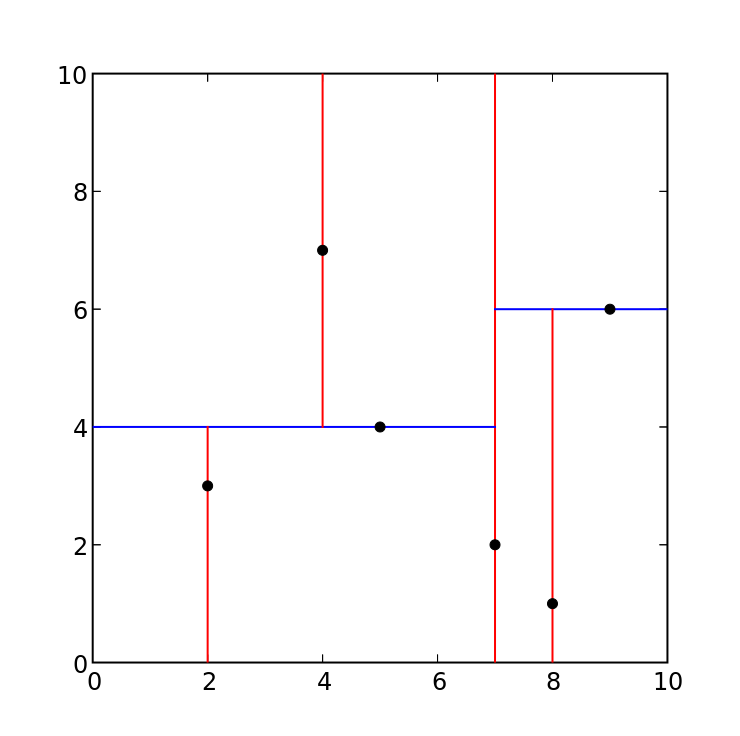
\includegraphics[width=7cm]{img/kdtree-plane.png}}
\caption{Разбиение плоскости на области с помощью k-d-дерева. Первое разбиение делается по x-координате относительно точки (7;2), чему соответствует вертикальная красная прямая при $x=7$.}
\label{ris:kdplane}
\end{figure}
\begin{figure}[H]
\center{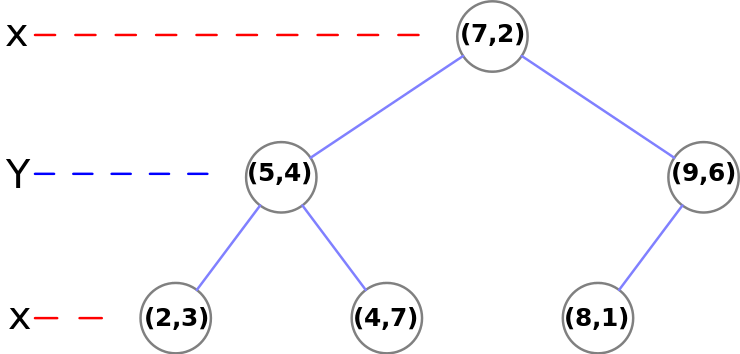
\includegraphics[width=7cm]{img/kdtree-tree.png}}
\caption{Структура k-d-дерева для приведенного выше набора точек. Можно видеть, что глубина такого дерева равна трем, хотя подобное дерево создает 7 отличающихся областей.}
\label{ris:kdtree}
\end{figure}
\end{center}


Чтобы сделать поиск объекта, нужно <<спуститься>> вектором по дереву (\cref{ris:annoy_tree}), определяя функцию на каждом уровне и делая сравнение с разделяющей вершиной. Это определит позицию вектора в дереве. Для поиска k соседей кроме позиции нужно найти некоторую окрестность, результаты в которой считаются позволительными. Обычно для этого предлагается следующее решение --- при спуске по дереву алгоритм может сделать рекурсивный поиск у обоих сыновей вершины, если вектор запроса имел значение функции, близкое к значению разделяющего вектора. Это эквивалентно тому, чтобы сделать запрос поиска для каждой точки из некоторой окрестности вектора запроса.

\begin{center}
\begin{figure}[H]
\center{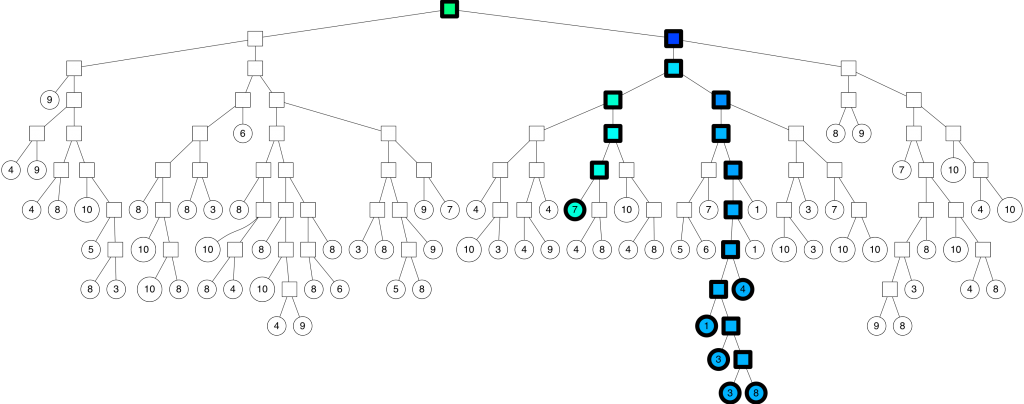
\includegraphics[width=10cm]{img/annoy_tree.png}}
\caption{Запрос на подмножестве поискового дерева рассматривает разных соседей одной вершины для продолжения поиска.}
\label{ris:annoy_tree}
\end{figure}
\end{center}

К достоинствам этого класса алгоритмов относится наглядность, возможность динамически менять поисковый индекс. Но, как правило, такие алгоритмы плохо работают для векторов больших размерностей, потому что неявно оставляют только $O(\log n)$ отличительных признаков у каждого объекта.

\subsection{Алгоритмы на основе хеширования}

\paragraph{LSH}

\label{LSH}

Идея алгоритма LSH \cite{gionis1999similarity} в том, чтобы отсечь все <<непохожие векторы>> с помощью $k$ случайных хеш-функций. Более конкретно, для заданной задачи выбирается специальное семейство хеш-функций $H$, из которого выбирается $k$ случайных хеш-функций. Часто хеш-функции являются бинарными, за счет чего из полученных $k$ значений можно сформировать одно новое число. Объекты считаются одинаковыми, если все значения хеш-функций совпали (\cref{ris:lsh_hashtable}). В некоторых вариациях алгоритма совпасть должны не все значения, а некоторая доля. Таким образом, при поиске достаточно рассматривать элементы, имеющие такое же значение хеш-функции, как и у искомого вектора.


\begin{center}
\begin{figure}[H]
\center{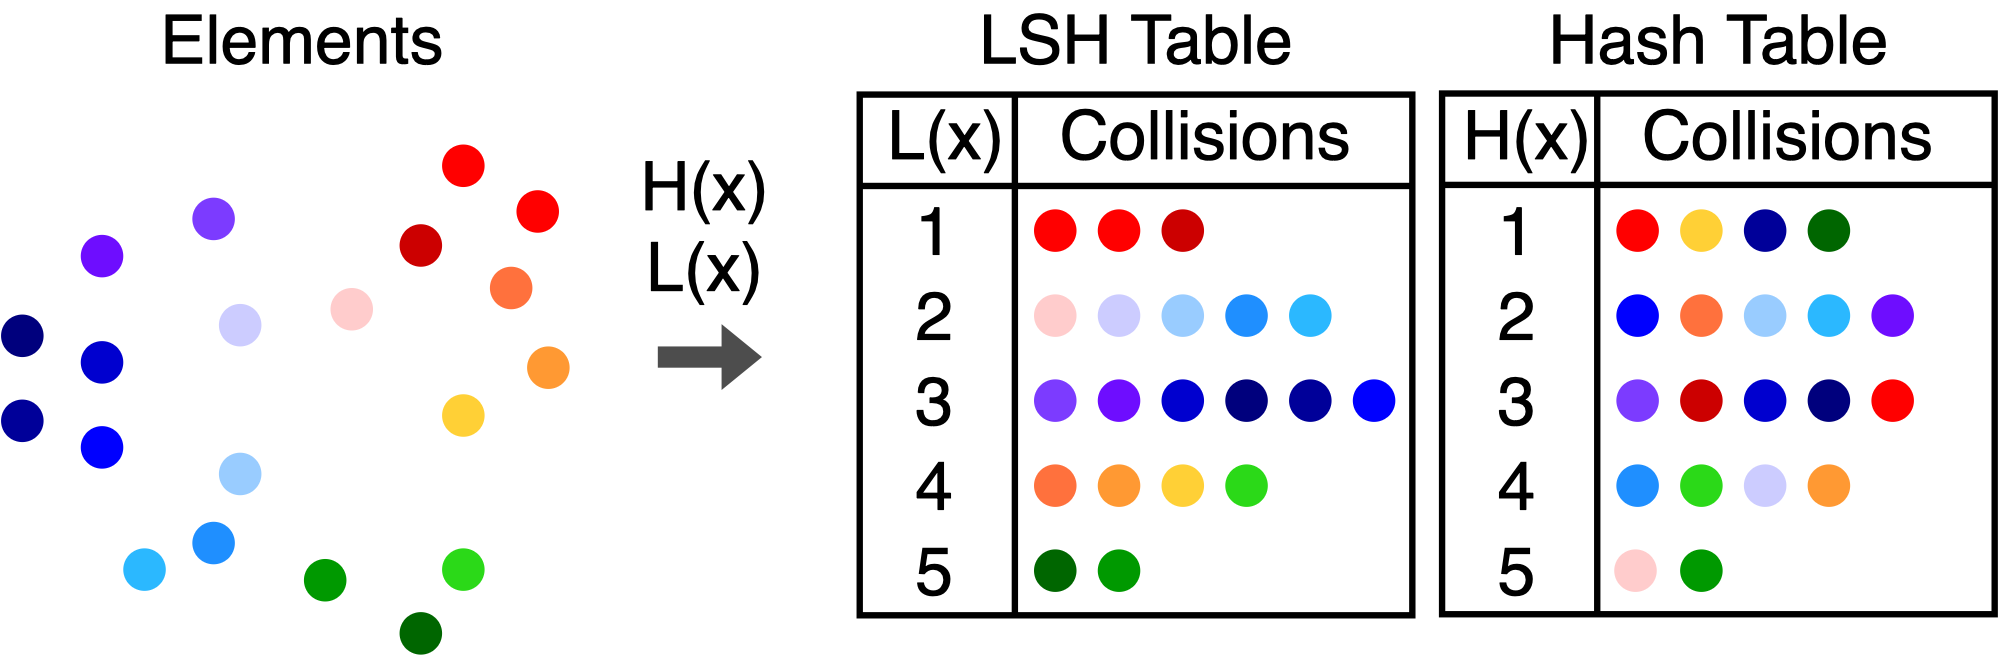
\includegraphics[width=10cm]{img/lsh_hashtable.png}}
\caption{Хеш-функция LSH для красных, похожих, объектов имеет значение 1, в то время, как для обычной хеш-функции красные объекты распределяются случайно.}
\label{ris:lsh_hashtable}
\end{figure}
\end{center}


Примером LSH-функции для бинарных векторов и расстояния Хэмминга может быть отдельно взятая координата: тогда при $k$ взятых координатах векторы с одинаковым значением хеш-функций имеют хотя бы $k$ общих бит --- а значит, метрика Хэмминга между такими векторами с большей вероятностью оптимальна, чем с теми объектами, где значение хеш-функции не совпало.

Для косинусного расстояния существует другое семейство LSH-функций: $h_i(x) = sgn (x, w_i)$, где $w_i$ --- случайная полуплоскость, проходящая через точку $0$. Тогда несколько полуплоскостей разбивают пространство на секторы, в каждом из которых лежат векторы с соседними углами (\cref{ris:lsh_cosine}).

Асимптотика для времени ответа на запрос и памяти для этих алгоритмов регулируемая и зависит от соотношения количества координат исходного вектора и количества хеш-функций.

\begin{center}
\begin{figure}[H]
\center{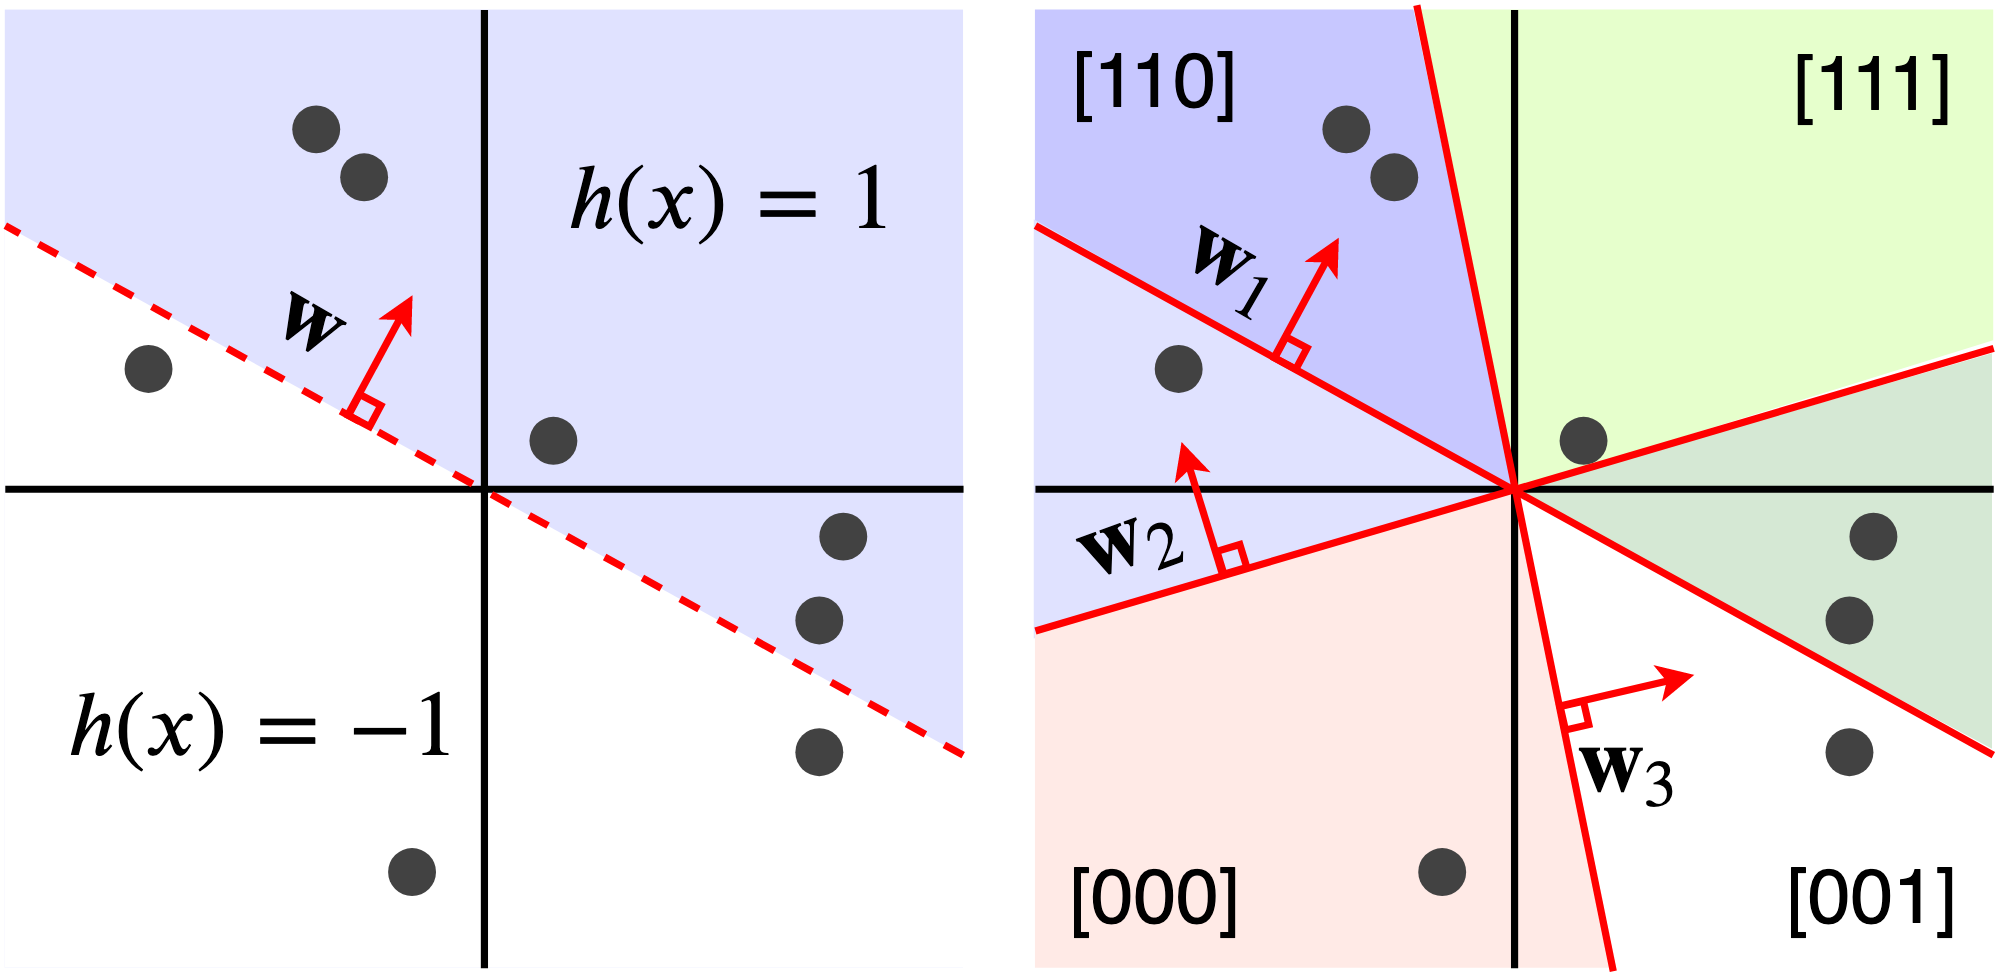
\includegraphics[width=10cm]{img/lsh_cosine.png}}
\caption{Объекты с близкими косинусными расстояниями окажутся в одинаковых областях. Например, область $[001]$ содержит все объекты, у которых $h_0(x) = -1, h_1(x) = -1, h_2(x) = 2$.}
\label{ris:lsh_cosine}
\end{figure}
\end{center}


Вариаций LSH очень много, данная работа \cite{jafari2021survey} делает обзор имеющихся результатов в сфере локального хеширования. Дополнительно опишем DMLSH, как метод, позволяющий обновлять поисковый индекс динамически.

\paragraph{DMLSH.}
Это алгоритм, представленный в 2013, который умеет динамически менять поисковый индекс \cite{yin2013dynamic}. Авторы алгоритма предлагают строить индекс <<на ходу>>, постепенно добавляя в индекс новые хеш-функции. Такой алгоритм помогает решать задачу $c$-$k$-ANN динамически с помощью локального хеширования.

Структура DMLSH строит дерево (\cref{ris:dmlsh}), аналогичное k-d-дереву, но строит его не над пространством $\mathbb{R}^d$, а над пространством значений хеш-функций. Если вершина дерева соответствует большому числу объектов, вершина создает новые листья, добавляя еще одну lsh-функцию. 

\begin{center}
\begin{figure}[H]
\center{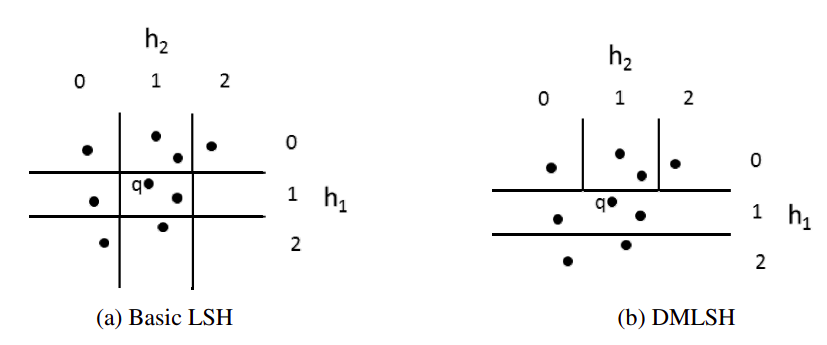
\includegraphics[width=10cm]{img/dmlsh.png}}
\caption{DMLSH не создает хеш-функции без необходимости, за счет чего поисковый индекс можно менять динамически. На картинке добавлять вторую хеш-функцию $h_2$ нужно только для большой группы векторов с $h_1(v) = 0$.}
\label{ris:dmlsh}
\end{figure}
\end{center}

К сожалению, проверенной реализации DMLSH в открытом доступе найти не получилось. Тем не менее, у LSH есть многообещающая возможность гибко настраивать количество хеш-функций, за счет чего поиск может работать очень быстро.

\subsection{Алгоритмы на основе квантизации}

\label{QUANT}

Этот класс алгоритмов <<сжимает>> пространство, в котором ведется поиск. А именно, пространство $\mathbb{R}^d$ меняется на $C \subset \mathbb{R}^d, |C| = k \in \mathbb{N}$. Точки в новом пространстве называются центроидами. Исходному вектору $x$ в соответствие ставится ближайший центроид $q(x) \stackrel{\text{def}}{=} \displaystyle \argmin_{c \in C} dist(c, x)$ (\cref{ris:voronoi}). Таким образом, для каждого объекта достаточно хранить номер центроида, который занимает $\log k$ бит. Если кроме номера центроида для каждой вершины сохранить расстояние до центроида, то можно хранить сжатое множество, с небольшой потерей точности~--- теперь любой поиск расстояния: $dist(A, B) \simeq dist(A, q(B)) + dist(q(B), B)$ (\cref{ris:loss_quant}).

\begin{center}
\begin{figure}[H]
\center{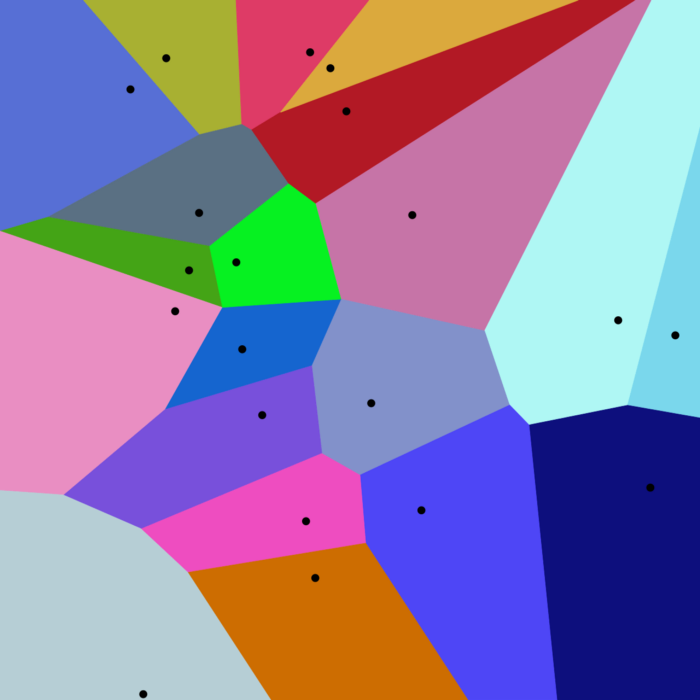
\includegraphics[width=5cm]{img/voronoi.png}}
\caption{Точками обозначены центроиды, а цветными областями разделены точки, соответствующие разным центроидам. Такая конструкция называется диаграмой Вороного}
\label{ris:voronoi}
\end{figure}
\end{center}

\begin{center}
\begin{figure}[H]
\center{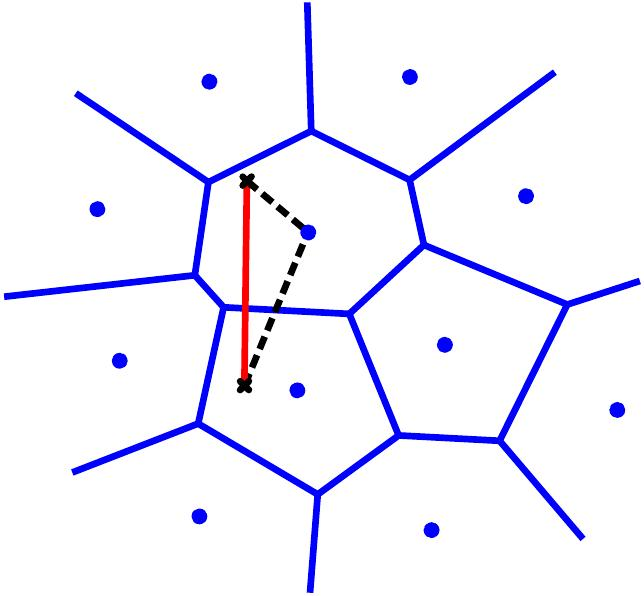
\includegraphics[width=5cm]{img/quantization_acc_loss.jpg}}
\caption{Поиск расстояния теряет некоторую точность, потому что одна сторона треугольника меньше, чем сумма двух других.}
\label{ris:loss_quant}
\end{figure}
\end{center}

Разные алгоритмы для квантизации предлагают разные функции $q(x)$. Самая простая такая функция может находиться с помощью алгоритма K-means методом выделения кластеров в данных (\cref{ris:kmeans}). Центром кластера становится новый квант. Такой метод плохо применим, когда кластеров много, поэтому нужно рассмотреть другие техники.

\begin{center}
\begin{figure}[H]
\center{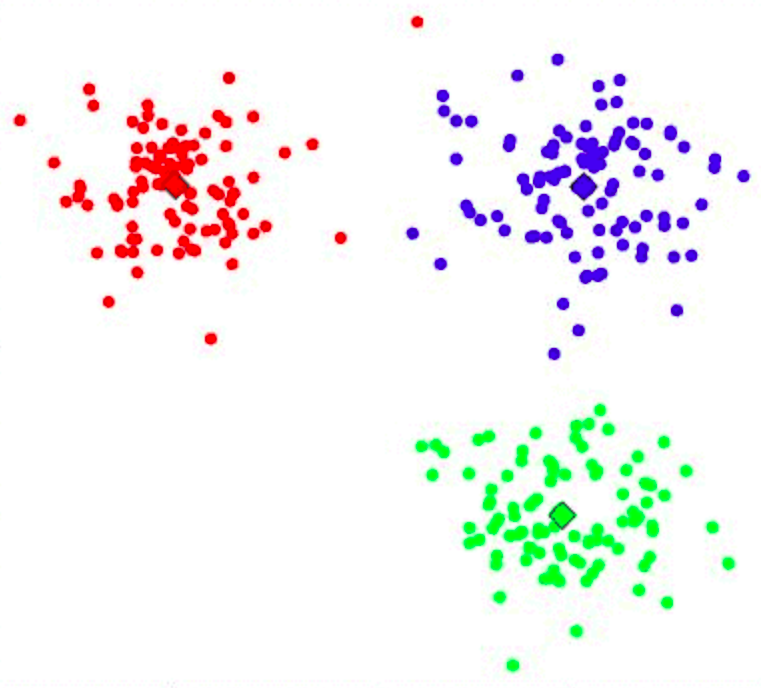
\includegraphics[width=5cm]{img/cluster_quant.png}}
\caption{Квантизация с помощью K-means}
\label{ris:kmeans}
\end{figure}
\end{center}

Метод Product Quantization ищет центроиды не для всего вектора размера $d$, а для его подвекторов меньших размеров. Затем полученные центроиды связывают вместе, создавая сетчатую структуру (\cref{ris:pq}). Таким образом, задачу кластеризации требуется решать на пространстве меньшей размерности, а при объединении количество доступных центроидов заметно увеличивается, не требуя дополнительной памяти.

\begin{center}
\begin{figure}[H]
\center{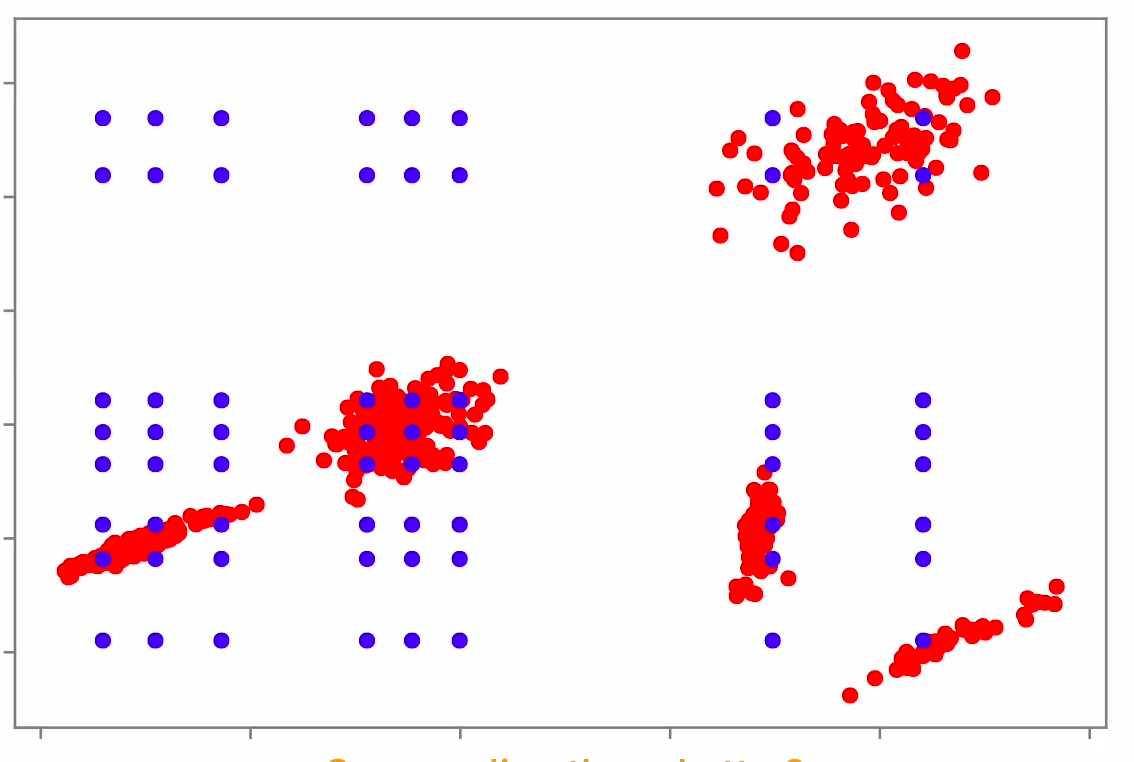
\includegraphics[width=7cm]{img/product_quant.png}}
\caption{Определение центроидов для Product Quantization. Синие центроиды были получены как декартово произведение центроидов по x-коордиинате и центроидов по y-координате}
\label{ris:pq}
\end{figure}
\end{center}

К сожалению, у данного метода не получилось найти вариации, применимые в динамической постановке задачи. Это можно объяснить тем, что алгоритме на основе квантизации опираются на найденные центроиды, а изменение базы может достаточно сильно повлиять на множество центроидов.

\subsection{HNSW}
\label{HNSW}


Алгоритм HNSW \cite{DBLP:journals/corr/MalkovY16} строит граф связей между соседними объектами в несколько уровней~--- на верних уровнях находится меньшее количество объектов, на нижних находится большее количество. Вектору соответствует вершина в графе. Каждая вершина соединена с $k$ соседями. При запросе на поиск ближайшего поиска используется алгоритм локальной оптимизации \cite{hnwspics}. А именно, если у заданной вершины есть сосед с меньшим расстоянием до искомого вектора, то алгоритм переходит к заданной вершине. Если такого соседа нет, то алгоритм переходит на более низкий уровень и продолжает поиск (\cref{ris:hnsw_graph}). В полученной структуре данных можно производить динамическое обновление индекса.

\begin{center}
\begin{figure}[H]
\center{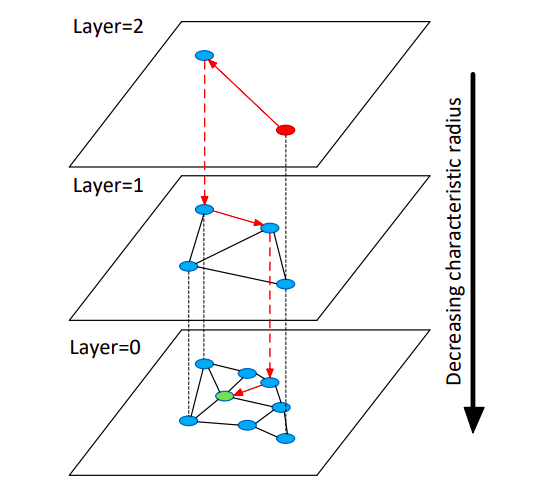
\includegraphics[width=7cm]{img/hnsw_graph.png}}
\caption{Структура слоистого графа в алгоритме HNSW. При запросе поиска алгоритм делает поиск по слоям~--- сначала на первом слое находится самая близкая вершина, а затем делается переход на следующий слой.}
\label{ris:hnsw_graph}
\end{figure}
\end{center}

\subsection{Сравнение алгоритмов}

При сравнении алгоритмов по основным критериям: времени обработки запросов, требуемой памяти, возможности динамической работы, получилась таблица для четырех рассмотренных подходов (\cref{tab:ann_comp}).

\begin{figure}[H]
\centering
\captionof{table}{Сравнение ANN-алгоритмов \cite{lopq}. Размер базы $n$, размер одного вектора $d$, количество центроидов $q$. За $T_h$ обозначим время работы lsh-функции $h: \mathbb{R}^d \to \mathbb{R}^k$}
\label{tab:ann_comp}
\begin{tabular}{|c|c|c|c|c|}
\hline
     & Время &  Память & Динамический? & Комментарий \\
     \hline
    K-D \ref{KD}& $O(d \log n)$ & $O(nd)$ & да & лучше маленькие $d$ \\
    \hline
    Квантизация \ref{QUANT} & $O(qd)$ & $O(qd + n \log q)$ & нет & потеря точности \\
    \hline
    LSH \ref{LSH}& $O(T_h \log n)$ & $O(nk)$ & да & \\
    \hline
    HNSW \ref{HNSW} & $O(d\log n)$ & $O(nd)$ & да & \\
    \hline
\end{tabular}
\end{figure}

Считая, что в SimSearch векторы редко бывают небольшого размера, HNSW оказывается предпочтительнее K-d деревьев. Квантизация не дает динамически обновлять базу данных и теряет в точности. Таким образом, есть смысл в первую очередь добавить стратегии на основе LSH и HNSW.

\subsection{Изученные библиотеки}

Были изучены крупные библиотеки с открытым исходным кодом, покрывающие различные подходы к решению задачи $c$-$k$-ANN. Среди критериев для выбора (которым подошли не все библиотеки), были:

\begin{itemize}
\item Наличие нескольких вариаций поискового алгоритма в одной библиотеке.
\item Возможность подключения в проект на C++.
\item Приемлемое время работы.
\end{itemize}

\paragraph{Annoy.}
Библиотека от Spotify \cite{Github:annoy}, использующая в своем ядре KD-дерево (\cref{ris:annoy_plane}). Авторы отмечают, что библиотека заточена под векторы небольшой размерности, но применять ее можно и при больших размерностях. Библиотека поддерживает C++/Python.

\begin{center}
\begin{figure}[H]
\center{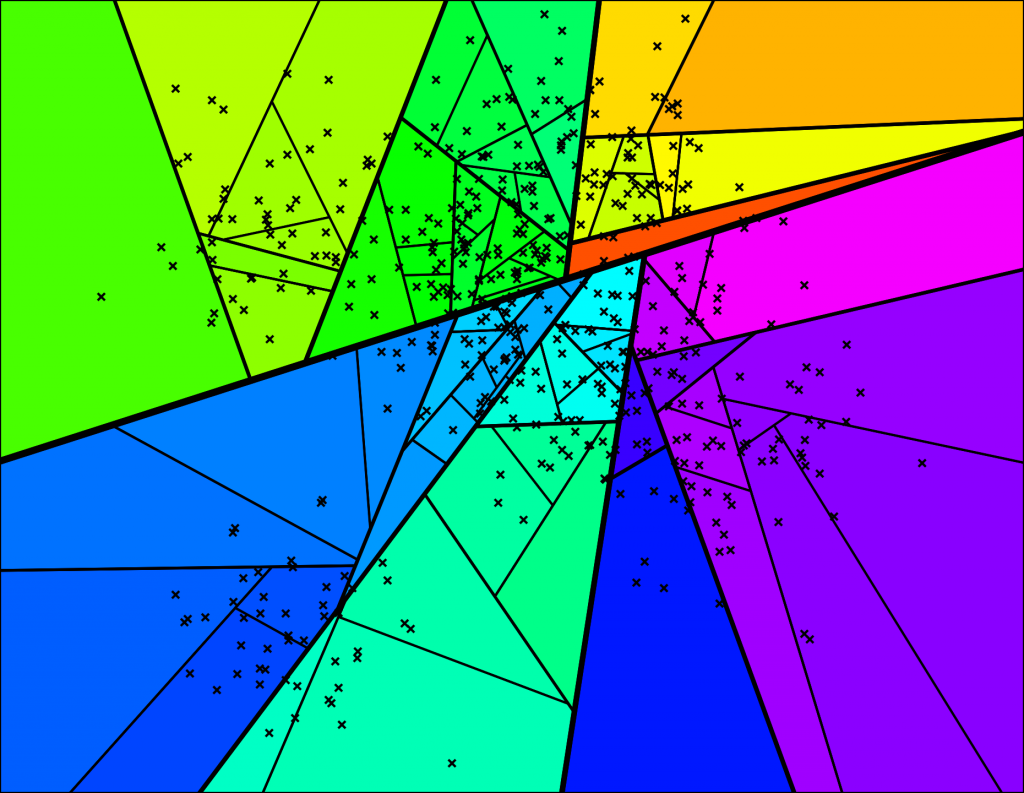
\includegraphics[width=6cm]{img/annoy_plane.png}}
\caption{Разбиение плоскости до листьев дерева в annoy}
\label{ris:annoy_plane}
\end{figure}
\end{center}

\paragraph{LSHKIT.} LSHKit \cite{lshkit}~--- библиотека от автора статьи про LSH \cite{dong2008modeling}. Библиотека поддерживает несколько видов расстояний и реализует LSH <<как из статьи>>, с возможностью кастомизировать алгоритм под требуемую функцию расстояния. LSHKit не поддерживает динамическое обновление индекса. Динамический индекс для LSH не получилось найти в open-source, только в статьях. Библиотека поддерживает C++.

\paragraph{ScaNN.}

ScaNN \cite{Github:scann}--- библиотека от Google, выпущенная в 2020 году \cite{guo2020accelerating}. Эта библиотека используют специальную функцию потерь для определения центроида в группе, показывает state-of-the-art результаты. Библиотека поддерживает Python, но исходный код написан на C++, так что теоретическая возможность добавления в проект есть.

\paragraph{FaiSS.}
FaiSS \cite{Github:faiss}--- библиотека от Facebook, выпущенная в 2017 году \cite{johnson2019billion}. Библиотека использует большое количество инженерных решений, в частности умеет работать с GPU. Большим преимуществом этой библиотеки является большое количество реализованных алгоритмов: HNSW, LSH, Quantizer. Библиотека поддерживает C++/Python.

\paragraph{DiskANN.} Библиотека от Microsoft, которая реализует графовые поисковые алгоритмы, явлюящиеся некоторым продолжением HNSW \cite{jayaram2019diskann}. Библиотека поддерживает C++.

\paragraph{NMSLib.} Библиотека NMSLib \cite{Github:nmslib} используется в ElasticSearch \cite{DBLP:conf/sisap/BoytsovN13} \cite{elasticsearch}. Эта библиотека, с одной стороны, реализует сразу несколько высокопроизводительных алгоритмов поиска; с другой стороны, их алгоритмы подходят для не-метрических поисковых пространств. Библиотека поддерживает C++/Python.

\subsection{Сравнение библиотек}

Все приведенные работы так или иначе решают одну и ту же задачу, при этом не дают точного ответа на то, что и когда предпочтительнее использовать. Существует большое исследование производительности подобных библиотек на разных датасетах \cite{annbenchmark} (\cref{ris:benchmark}), но сделать вывод о тотальном доминировании одного из алгоритмов нельзя, потому что многое зависит от характера нагрузки. Заметим также, что все сравнение основано не на абстрактной скорости, а на queries per second относительно полноты поиска.

\begin{center}
\begin{figure}[H]
\center{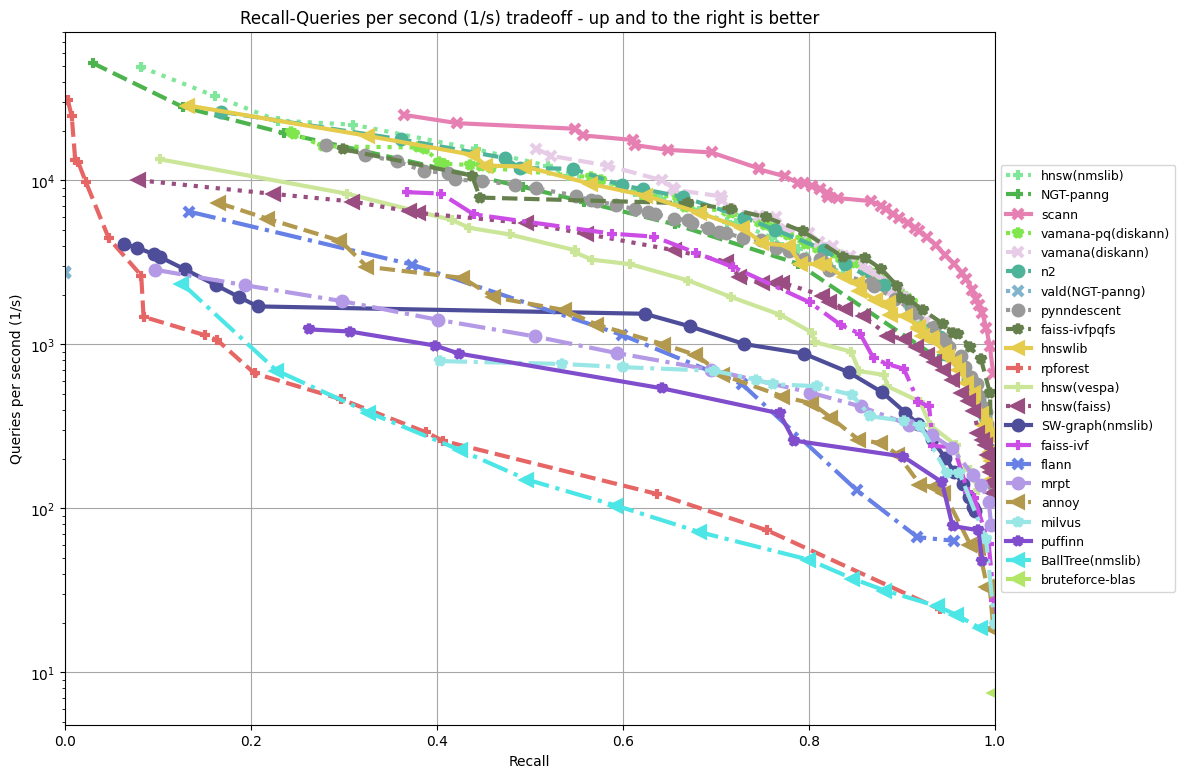
\includegraphics[width=15 cm]{img/glove-100-angular_10_angular.png}}
\caption{Результат сравнения библиотек для решения задачи ANN \cite{annbenchmark} (тест glove-100-angular, делался поиск 10 ближайших векторов). Тестирование проводилось на L2-метрике (то есть, оптимизировалось Евклидово расстояние). Разные конфигурации DiskANN, ScaNN, Nmslib, Faiss в списке лучших.}
\label{ris:benchmark}
\end{figure}
\end{center}

\subsection{Выводы}

Было принято решение добавить в SimSearch поисковую стратегию на основе линейного поиска для небольших объемов данных и тестирований поисковой выдачи, библиотеку Lshkit для LSH-алгоритма~--- LSHKit проверенная временем и небольшая, в будущем ее можно дополнить алгоритмом DMLSH. Помимо этого, она поддерживает различные расстояния, в частности расстояние Хемминга. Также была добавлена библиотека Faiss (HNSW) по двум соображениям~--- во-первых, Faiss предлагает множество стратегий (не только HNSW), во-вторых, это одна из лучших реализаций HNSW с открытым исходным кодом на C++ в исследовании ann-benchmark \cite{annbenchmark}, при условии поддержки динамического обновления индекса. В дальнейшем есть смысл добавить стратегии на основе квантизации и k-d-деревьев, а также реализовать DMLSH.

\newpage

\section {Реализация SimSearch}

SimSearch реализован как сервис на C++, предоставляющий API для решения поисковой задачи.

\subsection{API SimSearch}

SimSearch реализует HTTP REST API \cite{api}.

\begin{enumerate}

\item GET \begin{color}{blue}/status\end{color}~--- запрос статуса сервиса, возвращающий подтверждение, что все хранилища настроены и сервис работает. 
\item GET \begin{color}{blue}/search?id=ID\&storage=STORAGE\&n=N\end{color}~--- запрос поиска N объектов, похожих на объект ID, в хранилище STORAGE.
\item POST \begin{color}{blue}/search?storage=STORAGE\&n=N \end{color}~--- запрос поиска N объектов, похожего на объект, переданный в теле запроса, в хранилище STORAGE. Используется, если нужно передать метаинформацию для векторизатора.
\item POST \begin{color}{blue}/add?storage=STORAGE\end{color}~--- добавление объекта, переданного в теле запроса, в хранилище STORAGE.
\item POST \begin{color}{blue}/remove?storage=STORAGE\end{color}~--- удаление объекта, переданного в теле запроса, из хранилища STORAGE.

\end{enumerate}

\subsection{Архитектура SimSearch}

Сервис сделан на основе модели хранилищ и менеджера (\cref{ris:manager_storage}). Менеджер перенаправляет приходящие запросы к нужному хранилищу. Хранилище --- структура, содержащая информацию о данных в базе, а также \textit{векторизатор} и \textit{поисковую стратегию}. Векторизатор определяет правило перевода объекта в вектор (\ref{VECT}), а поисковая стратегия отвечает за решение задачи поиска соседних векторов (\ref{STRAT}). Векторизатор и стратегия поиска определяются независимо от конкретного хранилища. Таким образом, сервис получает возможность гибко определять ключевые части хранилища, не зависеть от логики других хранилищ, и переиспользовать код там, где это возможно.

\begin{center}
\begin{figure}[H]
\center{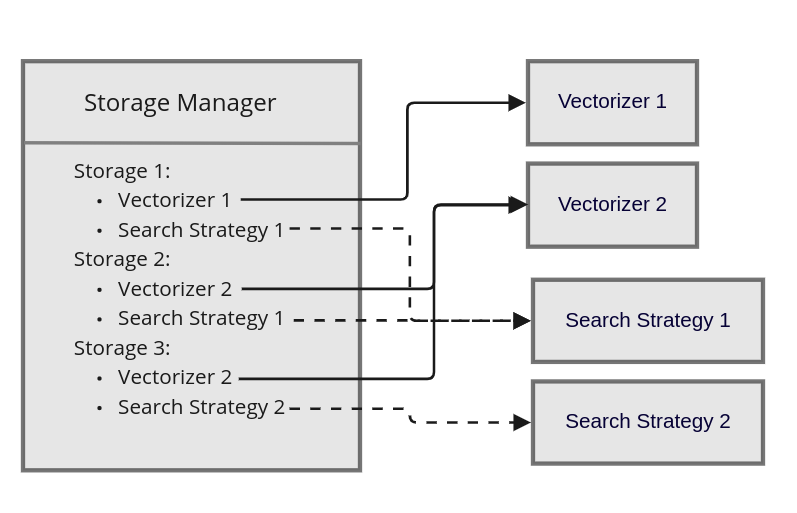
\includegraphics[width=7cm]{img/miro_3.png}}
\caption{Схема логики менеджер-хранилище. Можно видеть, что для трех хранилищ, которые суммарно используют 6 модулей, реализовать нужно всего 4 модуля, так как некоторые совпадают. Например, Vectorizer 2 используется и в Storage 2, и в Storage 3.}
\label{ris:manager_storage}
\end{figure}
\end{center}

Предполагается, что сервис поддерживает несколько методов векторизации по умолчанию, а необходимые пользователю сторонние методы выполняются либо на стороне пользователя, либо в интеграции с сервисом. Иначе говоря, в сервисе можно задать векторизаторы <<по умолчанию>>, а более сложные запросы придется реализовать на стороне клиента в удобном для пользователя формате. В таком случае хранилище потребует от пользователя обычные векторы.

Подобная структура не только сделает пользование сервисом гибким, но также позволит экспериментировать с алгоритмами поиска, так как заранее сложно предсказать, какой из предложенных алгоритмов покажет себя лучше всего. Также это даст возможность оптимизировать разные расстояния \ref{DIST} в зависимости от задачи \ref{SOLS}.

Опишем последовательность действий, которая используется SimSearch для обработки запросов (\cref{ris:architecture}):

\begin{enumerate}
\item Получить запрос от пользователя на API. Получить нужную информацию: идентификатор Storage, идентификатор объекта, метаинформацию объекта.
\item С помощью StorageManager получить объект Storage, который обработает запрос.
\item Storage получает из объекта вектор с помощью Vectorizer.
\item При работе с вектором есть два варианта:
\begin{enumerate}
\item При запросе поиска полученный вектор отдается в поисковую стратегию для получения поисковой выдачи.
\item При запросе модификации делается запрос изменения в Redis \cite{redis}, затем происходит обновление поискового индекса.
\end{enumerate}
\item Возвращается ответ на запрос.
\end{enumerate}

\begin{center}
\begin{figure}[H]
\center{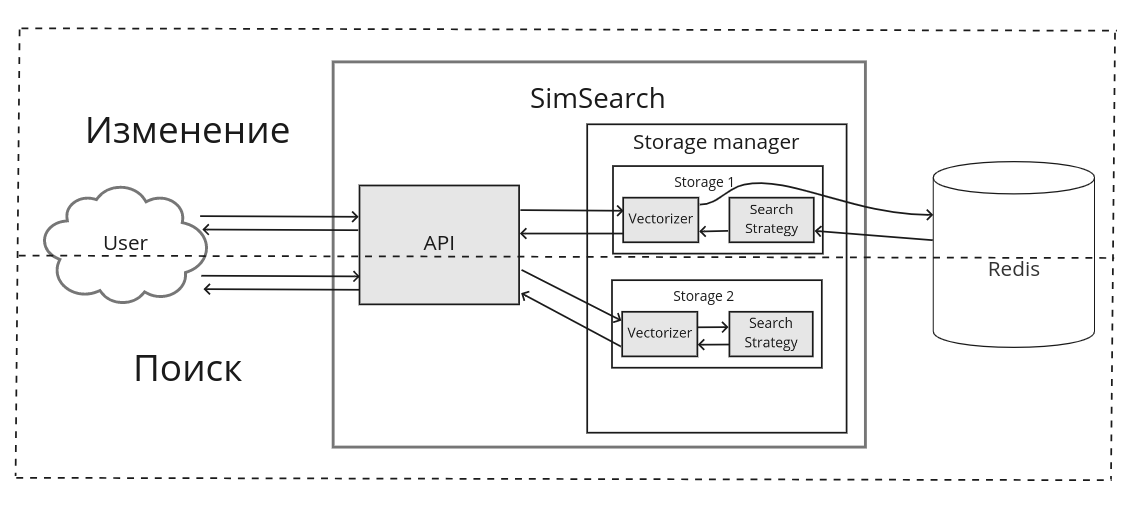
\includegraphics[width=15cm]{img/miro_4.png}}
\caption{Архитектура SimSearch, взаимодействие компонент при разных запросах.}
\label{ris:architecture}
\end{figure}
\end{center}



\subsection{Масштабирование}

Для того, чтобы приложение могло быть распределенным, нужно, чтобы данные хранились не в какой-то инсталляции хранилища, а в общей базе, к которой будут иметь доступ все серверы \cite{enwiki:1086236982}, на которых запущен SimSearch. Поисковый индекс хранилища, для разграничения логики, создается на каждом сервере \cite{enwiki:1086236982} независимо. Таким образом, нужно не только использовать базу данных, но и при обновлении объекта в базе обновлять поисковый индекс во всех инсталляциях. Для реализации такой логики был выбран Redis \cite{redis}, так как он предлагает и NoSQL базу данных в kv-формате, и поддерживает каналы для PUB-SUB взаимодействия \cite{pubsub}. Таким образом, в SimSearch Redis одновременно хранит базу данных в удобном формате и рассылает всем запущенным серверам \cite{enwiki:1086236982} SimSearch уведомление об изменении данных.

Когда какой-то сервер SimSearch получает запрос на обновление данных, узел делает обновление в таблице Redis, после чего с помощью очереди сообщений оповещает остальные сервера о изменении в данных (\cref{ris:scaling}).

\begin{center}
\begin{figure}[H]
\center{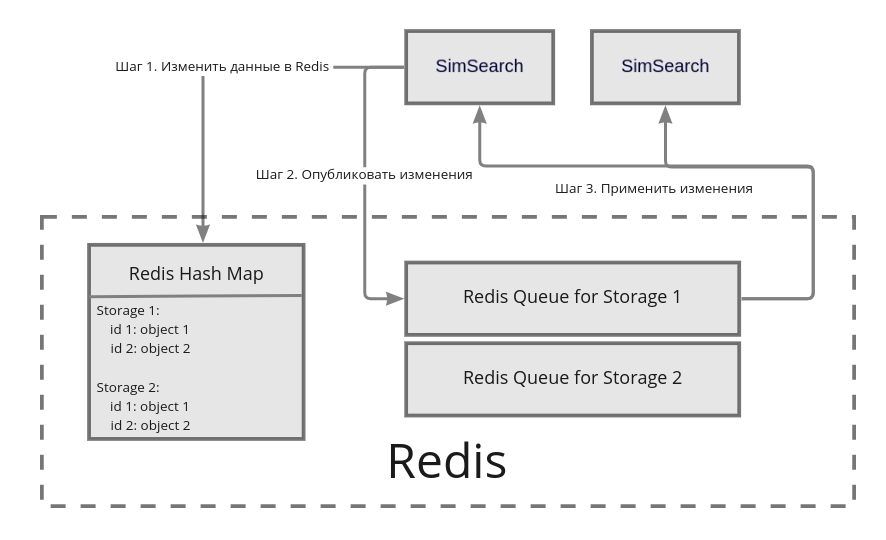
\includegraphics[width=12cm]{img/miro_1.png}}
\caption{Схема обновления данных между инсталляциями SimSearch с помощью Redis.}
\label{ris:scaling}
\end{figure}
\end{center}

\subsection{Объект поиска}

Объект поиска для SimSearch --- это структура, имеющая:
\begin{itemize}
\item Некоторый строковый идентификатор (например, в качестве идентификатора изображения может выступить его url).
\item Векторное представление (предполагается, что вектор содержит либо bool, либо float).
\item Поле, которое используется для хранения метаинформации объекта. \\ Метаинформация может как использоваться Vectorizer-ом для эмбединга, так и храниться для внешнего использования.
\end{itemize}


Внутри SimSearch объект поиска хранится в своем JSON-представлении (\cref{ris:json_eufel}).

\begin{center}
\begin{figure}[H]
\center{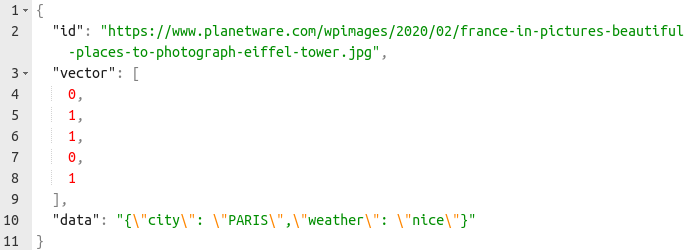
\includegraphics[width=10cm]{img/json_object.png}}
\caption{Представление изображения Эйфелевой башни \cite{parispic} в виде json-объекта. Вектор сокращен для наглядности.}
\label{ris:json_eufel}
\end{figure}
\end{center}

\subsection{Storage Manager}

Storage Manager решает две задачи:

\begin{enumerate}
    \item Настроить хранилища на основе конфигурационного файла сервиса.
    \item Передать пришедший запрос нужному хранилищу. Запрос может прийти как от API, так и от subscriber-а Redis-а, в случае обновления какого-то хранилища.
\end{enumerate}

Таким образом, Storage Manager хранит хеш-таблицу, где хранилище хранится под своим именем. Для настройки хранилища менеджер достает из конфигурационного файла (\cref{ris:storages_configs}) стратегию поиска, стратегию векторизации, и задает их для хранилища.


\begin{center}
\begin{figure}[H]
\center{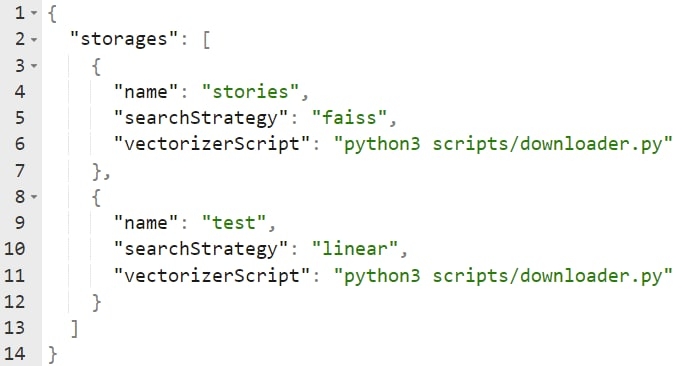
\includegraphics[width=8cm]{img/storages_configs.jpg}}
\caption{Конфигурация двух хранилищ: первое используется для поиска картинок, второе можно использовать для тестирования выдачи, поскольку линейный поиск находит оптимальные ответы.}
\label{ris:storages_configs}
\end{figure}
\end{center}


\subsection{Storage}

Storage реализует нужный интерфейс:

\begin{itemize}
\item Build: загрузить базу из Redis, построить поисковый индекс. Используется для инициализации.
\item Add: добавить объект в базу, обновить поисковый индекс. Если у поисковой стратегии нет реализации Add, обновить базу с нуля с помощью Build.
\item Remove: удалить объект из базы (если присутствует там), обновить поисковый индекс. Если у поисковой стратегии нет реализации Remove, обновить базу с нуля с помощью Build.
\item Search: Сделать поиск объекта в базе, вернуть $n$ ближайших по мнению стратегии векторов.
\end{itemize}

Storage осуществляет взаимодействие с Redis \cite{redis}, стратегией поиска и векторизатором. Логика Storage не зависит от стратегий поиска и векторизатора --- объект сначала векторизуется с помощью нужного Vectiorizer-а, а затем происходит либо поиск с помощью поискового ядра, либо обновление базы и запись в publisher Redis-а. Если Storage получает от менеджера обновление данных в Redis, то просит хранилище перестроиться соответствующим образом (\cref{ris:storage_logic}).

\begin{center}
\begin{figure}[H]
\center{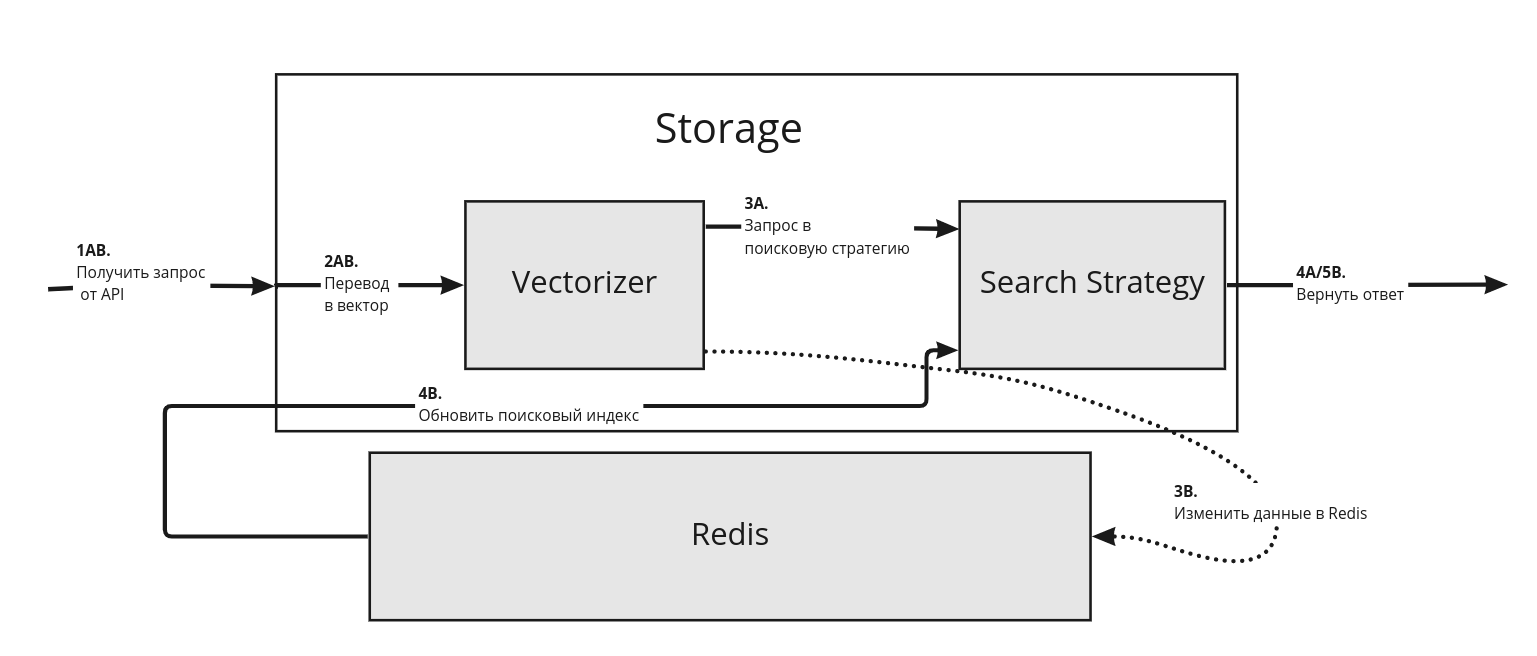
\includegraphics[width=16cm]{img/miro_2.png}}
\caption{Storage отвечает на зарос поиска (A) и обновления (B).}
\label{ris:storage_logic}
\end{figure}
\end{center}


\subsection{Vectorizer}

\label{VECT}

Vectorizer переводит объекты из описания в вектор. Реализуется одна функцию Transform, которая принимает объект и подсчитывает его вектор.

На текущий момент реализовано два Vectorizer'а:

\begin{enumerate}
    \item IdentityVectorizer: принимает объект, уже хранящий свой вектор в метаданных, возвращает вектор из объекта. Может использоваться, если пользователь уже сделал эмбеддинг без привязки к SimSearch.
    \item ScriptVectorizer, который запускает отдельным процессом скрипт, с которым взаимодействие идет через перенаправленные I/O-потоки. В скрипт передается строковое представление метаинформации объекта, в ответ скрипт возвращает текстовое представление векторного представления объекта. Примером реализованного ScriptVectorizer'а является скрипт, который переводит изображение в вектор, получая на вход url.
\end{enumerate}

\newpage
\subsection{Search}

\label{STRAT}

Поисковые стратегии --- одно из самых гибких мест в SimSearch. Разработчики сервиса могут добавить множество различных стратегий. Интерфейс стратегии покрывает следующие запросы:

\begin{itemize}
\item Запрос Search получает объект-запрос и параметр $n$ и возвращает $n$ объектов, которые по мнению стратегии являются самыми релевантными.

\item Запрос Add получает объект, который добавляется в поисковый индекс.

\item Запрос Remove удаляет объект, который был в поисковом индексе.
\end{itemize}

На текущий момент реализована стратегия линейного поиска, которая находит оптимальный ответ, стратегия поиска на основе lshkit с расстоянием Хемминга в качестве метрики, и стратегия на основе Faiss-HNSW. Стратегия на основе lshkit не поддерживает динамическое обновление хранилища, поэтому после каждого запроса изменения перестраивает его заново, что не подходит для динамической нагрузки, но подходит для нерегулярных изменений. 

В качестве примера, линейный поиск в рамках SimSearch реализован следующим образом:

\begin{itemize}
\item В качестве поискового индекса хранится динамический массив объектов.
\item При запросах обновления индекс добавляет/удаляет требуемый элемент.
\item При запросе поиска в индексе перебираются все объекты, с помощью кучи \cite{enwiki:1088468512} размера $k$ выбирается $k$ самых близких к искомому.
\end{itemize}

\subsection{Тестирование SimSearch}

Для SimSearch была настроена контейнеризация через Docker-образ \cite{docker}, а также docker-compose \cite{dockercompose} для сборки проекта в связке с Redis. Благодаря этому получилось создать изолированный экземпляр сервиса, который можно протестировать через публичное API.

\subsubsection{Тестирование корректности}

Было настроено автоматическое интеграционное тестирование проекта. Интеграционные тесты проверяют, что API сервиса начинает обрабатывать запросы, что запросы на добавление в пустую базу обрабатываются, и запросы на получения ближайших векторов получают непустой ответ. Интеграционные тесты реализованы на python с помощью pytest \cite{pytest}.
\newpage
Для проверки функционала написаны следующие тесты:
\begin{enumerate}
\item Создание непустой базы, проверка, что для объекта $x$ находится поисковая выдача.
\item Добавление объекта $x$ в базу, проверка, что он вернется в поисковой выдаче, как самый близкий.
\end{enumerate}

Помимо интеграционного тестирования с помощью pytest была реализована сборка проекта в GitLab CI/CD \cite{gitlab} и проверка тестов.

Таким образом, итоговая реализация SimSearch получилась готовой к использованию в реальных сервисах за счет сборки в GitLab CI/CD, сохранения docker-образа на удаленном GitLab сервере и выполнения на нем автоматического интеграционного тестирования.

\subsubsection{Тестирование производительности}

Для замеров производительности использовались тесты (\cref{tab:benchmark}), замеряющие время ответа на запрос Add/Search. Замерялись все реализованные поисковые стратегии, в качестве векторизатора использовался IdentityVectorizer, который не требует никакой обработки векторов, за счет чего замерялось именно время работы поисковых стратегий.

В качестве расстояний использовалось расстояние Хэмминга для стратегий linear и lshkit, для faiss-hnsw использовалось Евклидово расстояние. Поскольку эмбеддинг создавал бинарные вектора, минимизации этих двух метрик эквивалентны и они были выбраны, как стратегии по умолчанию для lshkit и faiss-hnsw.

\begin{figure}[H]
\centering
\captionof{table}{Тестирование различных поисковых стратегий.}
\label{tab:benchmark}
\begin{tabular}{|c|c|c|c|}
\hline
    Стратегия & Размер хранилища &  t(Add), мс & t(Search), мс \\
     \hline
    linear & 1000 & 12 & 98 \\
    \hline 
    linear & 5000 & 11 & 410 \\
    \hline 
    lshkit & 1000 & 89 & 14 \\
    \hline 
    lshkit & 5000 & 280 & 25 \\
    \hline 
    faiss-hnsw & 1000 & 12 & 43.5 \\
    \hline 
    faiss-hnsw & 5000 & 14 & 44 \\
    \hline 
\end{tabular}
\end{figure}

Видно, что сбалансированнее всего показала себя стратегия faiss-hnsw, поскольку стратегия одновременно динамическая и предлагает поиск за логарифмическое время. Можно заметить, что полученные результаты говорят о способности сервиса обрабатыавть несколько десятков запросов в секунду, что в первой версии сервиса для внутреннего пользования является более, чем достаточной пропускной способностью.

\newpage

\section{Поиск похожих картинок на основе SimSearch}

На основе SimSearch был разработан поиск похожих картинок. В качестве используемых картинок для поиска использовались фоновые изображения из <<историй>> (\cref{ris:story_1}) в финансовом мобильном приложении.

\begin{center}
\begin{figure}[H]
\center{
\includegraphics[width=3cm]{img/stories_1.png} 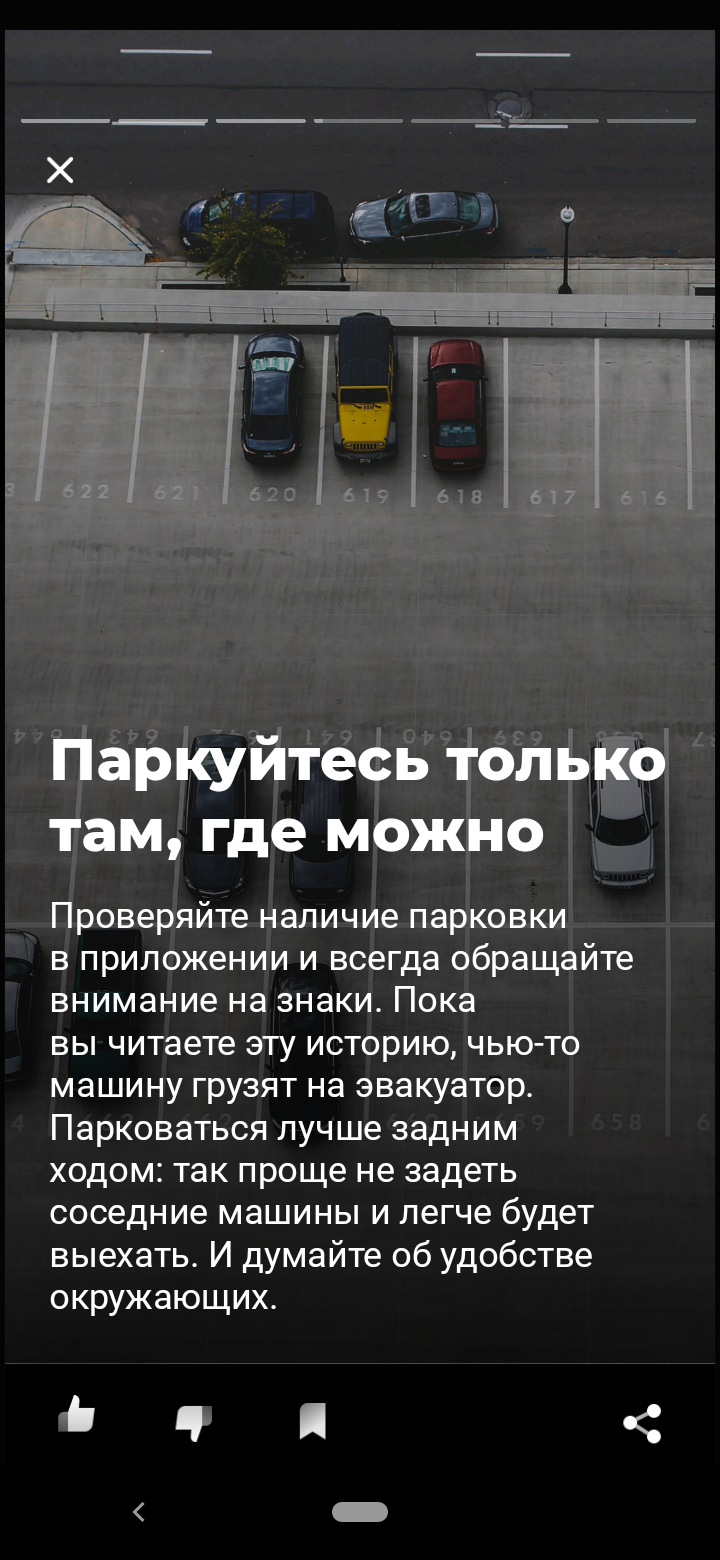
\includegraphics[width=3cm]{img/stories_2.png}}
\caption{Истории в мобильном финансовом приложении. Тематика произвольная, не привязана к финансам.}
\label{ris:story_1}
\end{figure}

\end{center}



Для разработки подобного веб-приложения нужно определиться с несколькими вопросами:
\begin{enumerate}
    \item Каким методом переводить объект в вектор?
    \item Какое расстояние использовать для сравнения векторов?
\end{enumerate}

Для перевода в вектор используется сверточная нейронная сеть, переводящая изображение в вектор. За основу взяты веса imagenet \cite{imagenet}. Таким образом, изображение переводится в вектор. За метрику взято расстояние Хэмминга. В качестве идентификатора изображений используется url.

Таким образом, веб-сервис для поиска изображений имеет очень простую логику: ему всего лишь нужно передавать запросы поиска в SimSearch, предварительно загрузив в него базу картинок. После этого нужно показать полученные результаты.

Для реализации веб-сервиса использовался flask \cite{flask}. Результаты получились впечатляющими: на относительно небольшой базе в 30000 изображений поиск находит достопримечательности, абстрактные объекты, кафе. Это хорошо решает задачу поиска картинок по референсам, потому что на базе таких размеров нужно искать не полное совпадение, достаточно что-то похожее по смыслу или внешнему виду.

\begin{center}
\begin{figure}[H]
\center{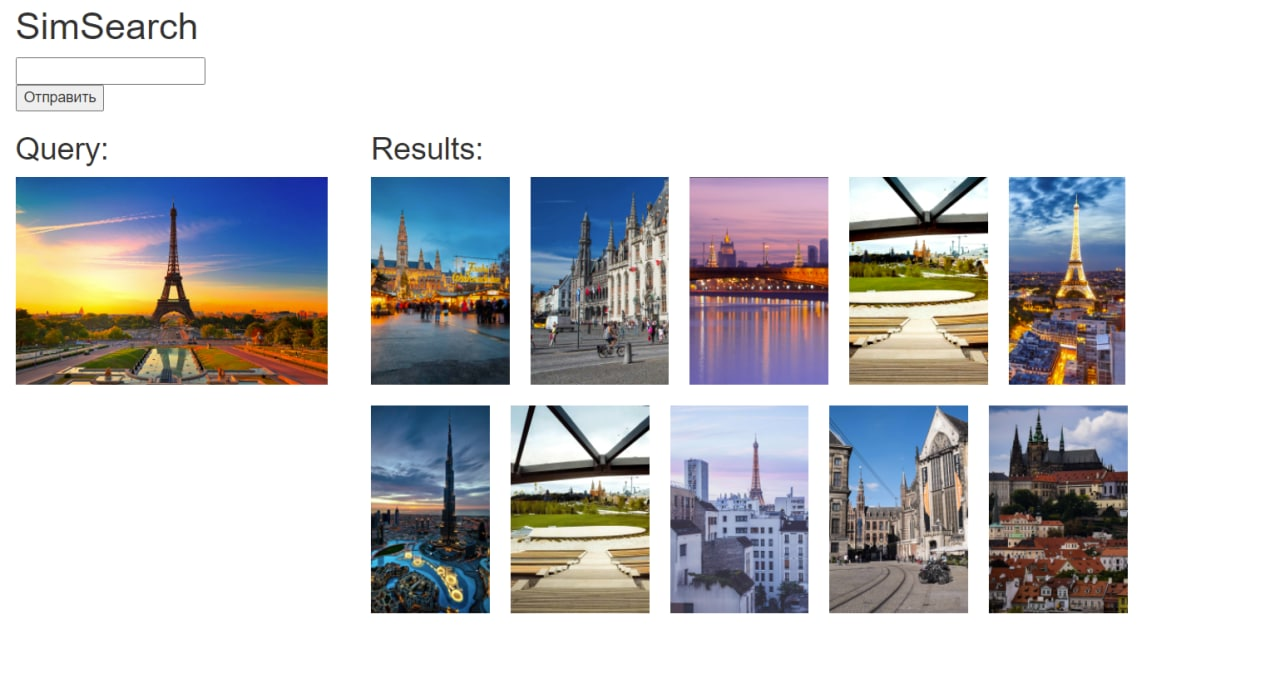
\includegraphics[width=15cm]{img/simsearch_paris.jpg}}
\caption{Поиск картинок, похожих на изображение Эйфелевой башни. Приложение находит изображения городов и достопримечательностей.}
\label{ris:simsearch_paris}
\end{figure}
\end{center}

\begin{center}
\begin{figure}[H]
\center{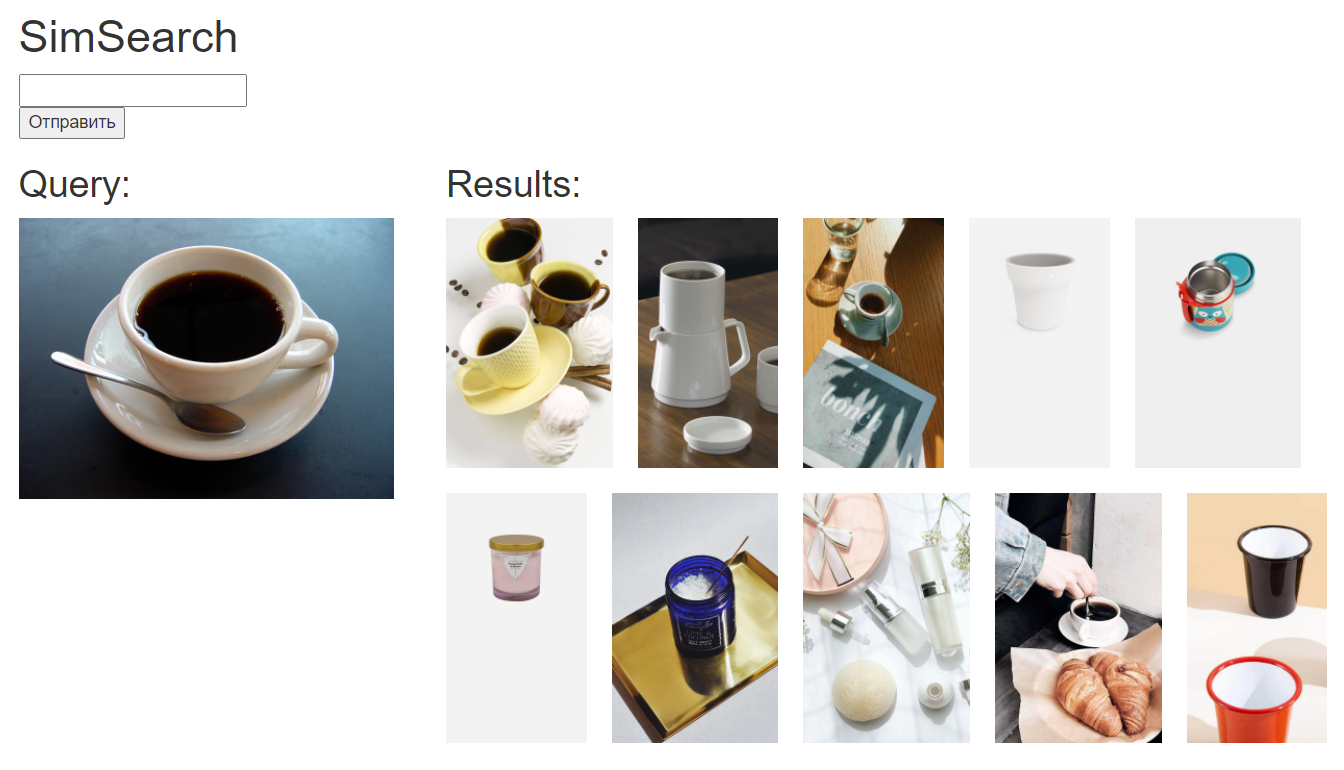
\includegraphics[width=15cm]{img/simsearch_coffee.png}}
\caption{Поиск картинок, связанных с кофе. Помимо кофе, можно найти разные кружки и даже круассаны!}
\label{ris:simsearch_coffee}
\end{figure}
\end{center}

\begin{center}  
\begin{figure}[H]
\center{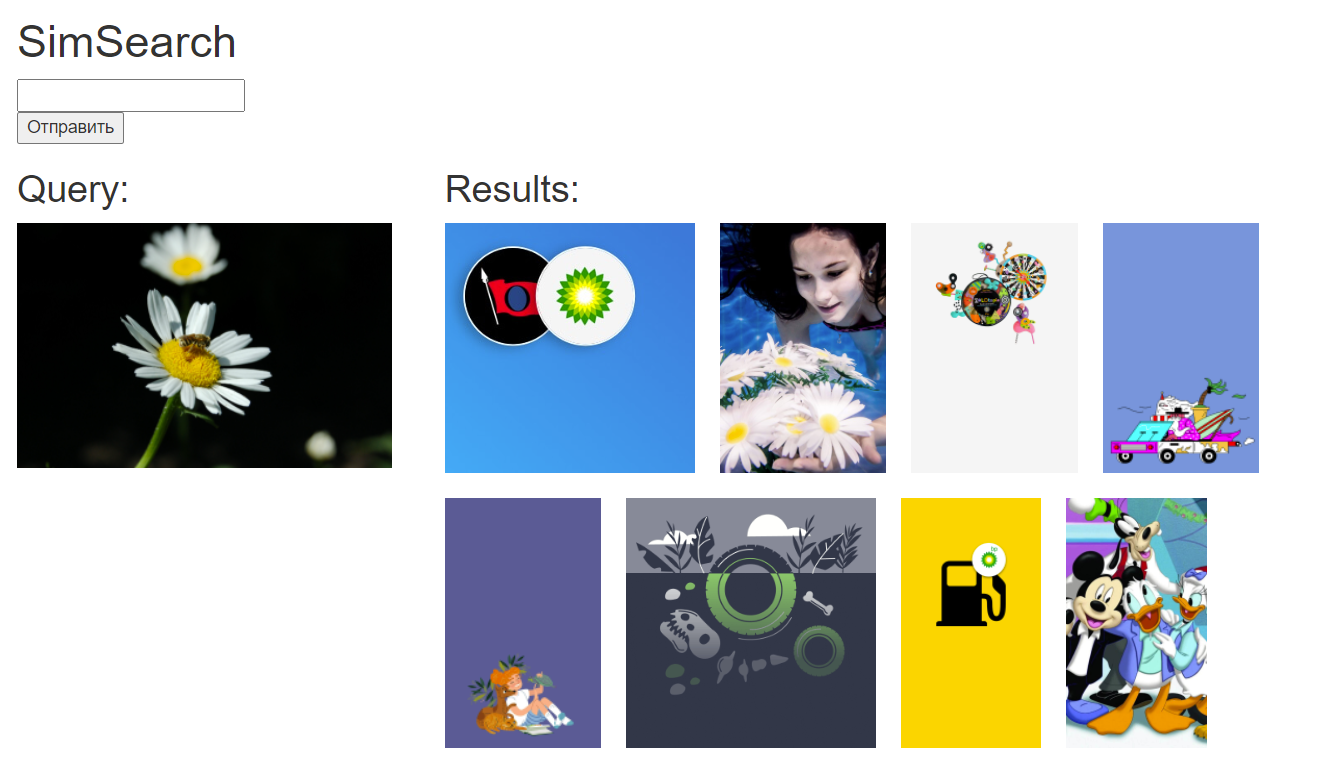
\includegraphics[width=15cm]{img/simsearch_daisy.png}}
\caption{Поскольку изображений с ромашками в базе почти нет, то находятся нерелевантные картинки и изображения с логотипом топливной компании, похожей на ромашку.}
\label{ris:simsearch_daisy}
\end{figure}
\end{center}

Приведем несколько примеров запросов. Для запросов достопримечательностей (\cref{ris:simsearch_paris}) и кофейной тематики (\cref{ris:simsearch_coffee}) находятся схожие изображения. Есть и менее удачные запросы поиска, где в базе не было нужных изображений, за счет чего результаты достаточно случайны (хоть и получилось найти зависимости между ромашкой и логотипом топливной компании, как на \cref{ris:simsearch_daisy}). 


\newpage

\section {Заключение}

Сформулируем, что было сделано в рамках курсовой работы, и какое дальнейшее развитие проекта возможно.

\subsection{Результаты}

В рамках курсовой работы был сделан сравнительный анализ алгоритмов для решения задачи $c$-$k$-ANN (K-d деревья \ref{KD}, LSH \ref{LSH}, квантизация \ref{QUANT}, HNSW \ref{HNSW}) и библиотеки (Annoy \cite{Github:annoy}, Nmslib \cite{Github:nmslib}, Faiss \cite{Github:faiss}, Scann \cite{Github:scann}, Lshkit \cite{lshkit}).

Был разработан сервис SimSearch, который можно использовать для поиска похожих объектов произвольного вида. SimSearch реализует HTTP REST API, выполняет векторизацию объекта и поиск ближайших векторов в базе, имеет возможность динамически менять базу. Для сервиса настроена контейнеризация и автоматическое интеграционное тестирование.

На основе сервиса SimSearch было создано приложение для поиска похожих изображений с UI интерфейсом, которое показывает релевантную поисковую выдачу.


\subsection{Дальнешее развитие}

Дальнейшее развитие работы заключается в исследовании новых поисковых алгоритмов и векторизаторов, а также в улучшении функционала сервиса SimSearch.

% \nocite{*}

\bibliographystyle{plain}
\bibliography{main}
	
	
\end{document}
